% ==============================================================================
% Modelo para Especificação de Projeto de Software
% Prof. Vítor E. Silva Souza - NEMO/UFES :: DI/UFES :: PPGI/UFES
%
% Baseado em abtex2-modelo-trabalho-academico.tex, v-1.9.2 laurocesar
% Copyright 2012-2014 by abnTeX2 group at http://abntex2.googlecode.com/ 
%
% This work may be distributed and/or modified under the conditions of the LaTeX 
% Project Public License, either version 1.3 of this license or (at your option) 
% any later version. The latest version of this license is in
% http://www.latex-project.org/lppl.txt.
%
% IMPORTANTE:
% Instruções encontram-se espalhadas pelo documento. Para facilitar sua leitura,
% tais instruções são precedidas por (*) -- utilize a função localizar do seu
% editor para passar por todas elas.
% ==============================================================================

% Usa o estilo abntex2, configurando detalhes de formatação e hifenização.
\documentclass[
	12pt,				
	oneside,		
	a4paper,			
	english,			% Idioma adicional para hifenização.
	french,				% Idioma adicional para hifenização.
	spanish,			% Idioma adicional para hifenização.
	brazil				% O último idioma é o principal do documento.
	]{abntex2}


%%% Importação de pacotes. %%%

% Conserta o erro "No room for a new \count". 
% O comando \reserveinserts deve ser comentado ou não, dependendo da versão do LaTeX.
\usepackage{etex}
%\reserveinserts{28}

% Usa a fonte Latin Modern.
\usepackage{lmodern}

% Seleção de códigos de fonte.
\usepackage[T1]{fontenc}

% Codificação do documento em Unicode.
\usepackage[utf8]{inputenc}

% Usado pela ficha catalográfica.
\usepackage{lastpage}

% Indenta o primeiro parágrafo de cada seção.
\usepackage{indentfirst}

% Controle das cores.
\usepackage[usenames,dvipsnames]{xcolor}

% Inclusão de gráficos.
\usepackage{graphicx}

% Tabularx package: melhor controle de leiaute de tabelas.
\usepackage{tabularx}

% Inclusão de páginas em PDF diretamente no documento (para uso nos apêndices).
\usepackage{pdfpages}

% Para melhorias de justificação.
\usepackage{microtype}

% Citações padrão ABNT.
\usepackage[brazilian,hyperpageref]{backref}
\usepackage[alf]{abntex2cite}	
\renewcommand{\backrefpagesname}{Citado na(s) página(s):~}		% Usado sem a opção hyperpageref de backref.
\renewcommand{\backref}{}										% Texto padrão antes do número das páginas.
\renewcommand*{\backrefalt}[4]{									% Define os textos da citação.
	\ifcase #1
		Nenhuma citação no texto.
	\or
		Citado na página #2.
	\else
		Citado #1 vezes nas páginas #2.
	\fi}

% \rm is deprecated and should not be used in a LaTeX2e document
% http://tex.stackexchange.com/questions/151897/always-textrm-never-rm-a-counterexample
\renewcommand{\rm}{\textrm}

% Inclusão de símbolos não padrão.
\usepackage{amssymb}
\usepackage{eurosym}

% Para utilizar \eqref para referenciar equações.
\usepackage{amsmath}

% Permite mostrar figuras muito largas em modo paisagem com \begin{sidewaysfigure} ao invés de \begin{figure}.
\usepackage{rotating}

% Permite customizar listas enumeradas/com marcadores.
\usepackage{enumitem}

% Permite inserir hiperlinks com \url{}.
\usepackage{bigfoot}
\usepackage{hyperref}

% Permite usar o comando \hl{} para evidenciar texto com fundo amarelo. Útil para chamar atenção a itens a fazer.
\usepackage{soulutf8}

%Colorir tabelas
\usepackage{colortbl}

% Colorinlistoftodos package: to insert colored comments so authors can collaborate on the content.
% (*) Indicar o nome do aluno e substituir o nome do professor se for o caso.
\usepackage[colorinlistoftodos, textwidth=20mm, textsize=footnotesize]{todonotes}
\newcommand{\aluno}[1]{\todo[author=\textbf{Aluno},color=green!30,caption={},inline]{#1}}
\newcommand{\vitor}[1]{\todo[author=\textbf{Vítor},color=red!30,caption={},inline]{#1}}

% Permite inserir espaço em branco condicional (incluído no texto final só se necessário) em macros.
\usepackage{xspace}

% Permite incluir listagens de código com o comando \lstinputlisting{}.
\usepackage{listings}
\usepackage{caption}
\DeclareCaptionFont{white}{\color{white}}
\DeclareCaptionFormat{listing}{\colorbox{gray}{\parbox{\textwidth}{#1#2#3}}}
\captionsetup[lstlisting]{format=listing,labelfont=white,textfont=white}
\renewcommand{\lstlistingname}{Listagem}
\definecolor{mygray}{rgb}{0.5,0.5,0.5}
\lstset{
	basicstyle=\scriptsize,
	breaklines=true,
	numbers=left,
	numbersep=5pt,
	numberstyle=\tiny\color{mygray}, 
	rulecolor=\color{black},
	showstringspaces=false,
	tabsize=2,
    inputencoding=utf8,
    extendedchars=true,
    literate=%
    {é}{{\'{e}}}1
    {è}{{\`{e}}}1
    {ê}{{\^{e}}}1
    {ë}{{\¨{e}}}1
    {É}{{\'{E}}}1
    {Ê}{{\^{E}}}1
    {û}{{\^{u}}}1
    {ù}{{\`{u}}}1
    {â}{{\^{a}}}1
    {à}{{\`{a}}}1
    {á}{{\'{a}}}1
    {ã}{{\~{a}}}1
    {Á}{{\'{A}}}1
    {Â}{{\^{A}}}1
    {Ã}{{\~{A}}}1
    {ç}{{\c{c}}}1
    {Ç}{{\c{C}}}1
    {õ}{{\~{o}}}1
    {ó}{{\'{o}}}1
    {ô}{{\^{o}}}1
    {Õ}{{\~{O}}}1
    {Ó}{{\'{O}}}1
    {Ô}{{\^{O}}}1
    {î}{{\^{i}}}1
    {Î}{{\^{I}}}1
    {í}{{\'{i}}}1
    {Í}{{\~{Í}}}1
}




%%% Definição de variáveis. %%%
% (*) Substituir os textos abaixo com as informações apropriadas.
\titulo{Aplicação do método FrameWeb no
desenvolvimento do sistema SCAP utilizando o
framework Grails}
\autor{Leonardo Nascimento dos Santos}
\local{Vitória, ES}
\data{2021}
\instituicao{
	Universidade Federal do Espírito Santo -- UFES
	\par
	Centro Tecnológico
	\par
	Departamento de Informática}
\newcommand{\subtitulo}{Documento de Projeto de Sistema}
\newcommand{\versao}{1.0}

% Define a capa.
% (*) Incluir linhas no registro de alterações a cada nova versão.
\renewcommand{\imprimircapa}{%
	\begin{capa}%
		\center
		
		{\ABNTEXchapterfont\large\subtitulo{}}
		\vfill
		\begin{center}
			\ABNTEXchapterfont\bfseries\LARGE\imprimirtitulo
		\end{center}
		
		\vfill
		Registro de Altera{\c c}{\~ o}es:
		\begin{table}[h]
			\centering
			\vspace{0.5cm}
			\begin{tabular}{|c|c|c|c|} \hline
			
 				Versão & Responsável & Data  & Alterações \\ \hline   
 				                            
				1.0  & \imprimirautor & 13/03/2019 & Versão Inicial  \\ \hline
				
				1.1  & \imprimirautor & 20/03/2021 & Modelos FrameWeb adicionados  \\ \hline  
			\end{tabular}
		\end{table}
		
		\vfill
		\large\imprimirlocal
		\linebreak
		\large\imprimirdata
		\vspace*{1cm}
	\end{capa}
}

% Macros específicas do trabalho.
% (*) Inclua aqui termos que são utilizados muitas vezes e que demandam formatação especial.
% Exemplo: Java com TM (trademark) em superscript.
% Use sempre \xspace para que o LaTeX inclua espaço em branco após a macro somente quando necessário.
\newcommand{\java}{Java\texttrademark\xspace}




%%% Configurações finais de aparência. %%%

% Altera o aspecto de algumas cores.
\definecolor{blue}{RGB}{41,5,195}
\definecolor{lightgray}{gray}{0.9}

% Informações do PDF.
\makeatletter
\hypersetup{
	pdftitle={\@title}, 
	pdfauthor={\@author},
	pdfsubject={\imprimirpreambulo},
	pdfcreator={LaTeX with abnTeX2},
	pdfkeywords={abnt}{latex}{abntex}{abntex2}{trabalho acadêmico}, 
	colorlinks=true,				% Colore os links (ao invés de usar caixas).
	linkcolor=blue,					% Cor dos links.
	citecolor=blue,					% Cor dos links na bibliografia.
	filecolor=magenta,				% Cor dos links de arquivo.
	urlcolor=blue,					% Cor das URLs.
	bookmarksdepth=4
}
\makeatother

% Espaçamentos entre linhas e parágrafos.
\setlength{\parindent}{1.3cm}
\setlength{\parskip}{0.2cm}



%%% Páginas iniciais do documento: capa, folha de rosto, ficha, resumo, tabelas, etc. %%%

% Compila o índice.
\makeindex

% Inicia o documento.
\begin{document}

% Retira espaço extra obsoleto entre as frases.
\frenchspacing

% Inclui o brasão da UFES.
\begin{figure}[h]
  \centering
  
\includegraphics[scale=0.055]{brasao.jpg}
  \label{ppts3}
\end{figure} 

% Capa do trabalho.
\imprimircapa





%%% Início da parte de conteúdo do documento. %%%
% Marca o início dos elementos textuais.
\textual

% Inclusão dos capítulos.
\begingroup
\let\clearpage\relax
% ==============================================================================
% TCC - Nome do Aluno
% Capítulo 1 - Introdução
% ==============================================================================
\chapter{Introdução}
\label{sec-intro}

Antigamente, os servidores não comportavam páginas \textit{Web} que continham um conteúdo muito denso. Funcionando apenas com páginas estáticas, realizar manutenções e controle das funcionalidades era uma tarefa muito difícil. Com o desenvolvimento de novas tecnologias a partir da criação da \textit{World Wide Web} (WWW) e através do surgimento de novas linguagens de programação para a \textit{Web}, os servidores tiveram que ser adaptados para se tornarem mais robustos. Com a infraestrutura de software modificada, os servidores começaram a aceitar páginas dinâmicas que passaram a ser carregadas de conteúdos que antes não eram suportados e isso também possibilitou que essas páginas possuíssem efeitos diversos, tais como animações de conteúdo.

Ainda nessa constante evolução, sistemas projetados para serem utilizados a partir de um navegador ou de aplicativos, puderam ser criados de uma maneira em que os servidores processassem e retornassem as informações para os visitantes através da Internet, surgindo assim o conceito de \textit{WebApp}, ou aplicação \textit{Web}. Lojas virtuais e sistemas de fornecimento entre empresas são exemplos de \textit{websites} que puderam ser desenvolvidos por meio de \textit{WebApps}. Desta maneira, o foco deste trabalho serão os Sistemas de Informação Baseados na \textit{Web (Web-based Information Systems – WISs)}, que são enquadrados em uma categoria específica de \textit{WebApps}. Esses sistemas são caracterizados como sistemas de informação tradicionais, mas estão disponíveis na Internet.

Quando falamos sobre o desenvolvimento de \textit{WebApps} atuais, em particular os WISs, temos que entender que utilizar a Engenharia de Software é uma tarefa fundamental. Os aspectos relacionados ao estabelecimento de técnicas, processos, métodos, ferramentas e ambientes de suporte ao desenvolvimento de software são tratados de forma clara pela Engenharia de Software~\cite{falbo:es14}. Trazendo alguns benefícios como, por exemplo, a compatibilidade entre plataformas e a facilidade de gerenciamento, as \textit{WebApps} por meio dos servidores, se tornaram indispensáveis para manterem os serviços e as aplicações disponíveis em qualquer parte do mundo através da Internet.

No meio de tantas criações e adaptações tecnológicas, surge o uso de \textit{frameworks} para \textit{WebApps}. Se tornando uma das ferramentas mais importantes para o desenvolvimento de \textit{WebApps}, os \textit{frameworks} passaram a auxiliar no encapsulamento das funcionalidades de alto nível com maior eficiência e agilidade, fazendo com que a maior parte do tempo e do trabalho fossem economizados. Visando propor uma abordagem diferenciada para a construção de sistemas para \textit{Web}, surge então o método FrameWeb (\textit{Framework-based Design Method for Web Engineering})~\cite{souza:masterthesis07}. Com o intuito de utilizar diversos \textit{frameworks}, o método FrameWeb busca agilizar o desenvolvimento de \textit{WebApps}, minimizando as tarefas realizadas nas fases que a Engenharia de Software determina.

Baseado na linguagem de modelagem UML (Unifield Modeling Language)~\cite{booch-et-al:u06}, o método FrameWeb propõe quatro diagramas para a fase de projeto de software que incorporam os conceitos trazidos pelos \textit{frameworks} utilizados no desenvolvimento Web, de modo a facilitar a comunicação entre desenvolvedores, agilizar o desenvolvimento por meio de geração de código, dentre outras vantagens. Originalmente, o método se propunha a dar suporte a três categorias de \textit{frameworks}: controladores frontais, injeção de dependências e mapeamento objeto/relacional.

Existem, no entanto, inúmeros \textit{frameworks} existentes dentro de cada categoria. Sendo assim, se faz necessário experimentar o método com \textit{frameworks} diversos, avaliando sua adequação. Neste contexto, \citeonline{duarte-pg14} desenvolveu uma \textit{WebApp} --- um Sistema de Controle de Afastamento de Professores (SCAP) --- em seu trabalho de conclusão de curso. Esse sistema foi criado para apoiar um departamento de universidade a realizar um controle das solicitações de afastamento de seus professores efetivos. Utilizando os requisitos que foram levantados por \citeonline{duarte-pg14} e posteriormente analisados por \citeonline{prado-pg15}, este trabalho tem com tarefa fundamental a implementação do SCAP utilizando dois outros \textit{frameworks Web}, para que seja possível realizar a verificação da eficiência do método FrameWeb.

Os \textit{frameworks} experimentados neste trabalho serão o GWT e o Grails. O \textit{framework} GWT foi desenvolvido utilizando a linguagem de programação Java como base e em sua construção, foi adicionado um kit de ferramentas de desenvolvimento que facilita a otimização e criação de \textit{WebApps} que utilizam Ajax. O \textit{framework} Grails utiliza as linguagens de programação Java e Groovy, tendo como característica a minimização da complexidade da criação de \textit{WebApps} e podendo ser integrado com qualquer biblioteca Java através de plugins.

%\hrulefill

%Além do template pronto para uso, este documento inclui exemplos de uso de \latex que podem ser úteis para aqueles que possuem pouca experiência com a ferramenta. Quando for começar a escrever seu PG, apague todo o conteúdo abaixo da palavra ``Texto''.



%%% Início de seção. %%%
\section{Seções e subseções}
\label{sec-intro-secoes}

O documento é organizado em capítulos (\texttt{\textbackslash chapter\{\}}), seções (\texttt{\textbackslash section\{\}}), subseções (\texttt{\textbackslash subsection\{\}}), sub-subseções (\texttt{\textbackslash subsubsection\{\}}) e assim por diante. Atenção, porém, a não criar estruturas muito profundas (sub-sub-sub-...) pois o documento não fica bem estruturado.


%%% Início de seção. %%%
\subsection{Referências a seções}
\label{sec-intro-secoes-refs}

Cada parte do documento (capítulo, seção, etc.) deve possuir um rótulo logo abaixo de sua definição. Por exemplo, este capítulo é definido com \texttt{\textbackslash chapter\{Introdução\}} seguido por \texttt{\textbackslash label\{sec-intro\}}. Assim, podemos fazer referências cruzadas usando o comando \texttt{\textbackslash ref\{rótulo\}}: ``O Capítulo~\ref{sec-intro} começa com a Seção~\ref{sec-intro-secoes}, que é ainda subdividida nas subseções~\ref{sec-intro-secoes-refs} e~\ref{sec-intro-secoes-sobrerefs}.

Para melhor organização das partes do documento, sugere-se primeiro utilizar o prefixo \texttt{sec-} (para diferenciar de referências à figuras, tabelas, etc. quando usarmos o comando \texttt{\textbackslash ref\{\}}) e também representar a hierarquia das seções nos rótulos. Por exemplo, o Capítulo~\ref{sec-intro} tem rótulo \texttt{sec-intro}, sua Seção~\ref{sec-intro-secoes} tem rótulo \texttt{sec-intro-secoes} e a Subseção~\ref{sec-intro-secoes-refs} tem rótulo \texttt{sec-intro-secoes-refs}.



%%% Início de seção. %%%
\subsection{Sobre referências cruzadas}
\label{sec-intro-secoes-sobrerefs}

Nas próximas seções, veremos que é possível fazer referência cruzada não só a seções mas também a listagens de código, figuras, tabelas, etc. Em todos estes casos, quando nos referimos à Seção X, Listagem Y ou Figura Z, consideramos que estes são os nomes próprios destes elementos e, portanto, usa-se a primeira letra maiúscula. Isso pode ser visto na Subseção~\ref{sec-intro-secoes-refs}, acima. A exceção é quando nos referimos a vários elementos ao mesmo tempo, por exemplo: ``as subseções~\ref{sec-intro-secoes-refs} e~\ref{sec-intro-secoes-sobrerefs}''.

Por fim, ao usar o comando \texttt{\textbackslash ref\{\}}, sugere-se separá-lo da palavra que vem antes dele com um \textasciitilde\ ao invés de espaço. Por exemplo: \texttt{o capítulo\textasciitilde \textbackslash ref\{sec-intro\}}. Isso faz com que o \latex não quebre linha entre a palavra \texttt{capítulo} e o número do capítulo.




%%% Início de seção. %%%
\section{Citações bibliográficas}
\label{sec-intro-citacoes}

Este documento utiliza a ferramenta de gerenciamento de referências bibliográficas do \latex, chamada \emph{BibTeX}. O arquivo \texttt{bibliografia.bib}, referenciado no arquivo \latex principal deste documento, contém algumas referências bibliográficas de exemplo. Assim como capítulos, seções, etc., tais referências também possuem rótulos, especificados como primeiro parâmetro de cada entrada (ex.: \texttt{@incollection\{souza-et-al:iism08, ...\}}.

Sugere-se um padrão para rótulos de referências bibliográficas para que fique claro também no código \latex qual referência está sendo citada. Por exemplo, ao citar a referência \texttt{souza-et-al:sesas13}, sabemos que é um artigo escrito por \emph{Souza} e outros, publicado no \emph{SESAS} em \emph{2013} (geralmente a pessoa que citou sabe que publicação é SESAS e quem é Souza).

Para citar uma referência bibliográfica contida no arquivo \emph{BibTeX}, basta usar seu rótulo como parâmetro de um de dois comandos possíveis de citação:

\begin{itemize}
	\item O comando \texttt{\textbackslash cite\{\}} efetua uma citação tradicional, colocando o nome do(s) autor(es) e o ano entre parênteses. Por exemplo, \texttt{\textbackslash cite\{souza-et-al:iism08\}} é transformado em \cite{souza-et-al:iism08};
	
	\item O comando \texttt{\textbackslash citeonline\{\}} efetua uma citação integrada ao texto, colocando o nome do(s) autor(es) direto no texto e somente o ano entre parênteses. Por exemplo, ``de acordo com \texttt{\textbackslash citeonline\{souza-et-al:iism08\}}'' é transformado em: de acordo com \citeonline{souza-et-al:iism08};
\end{itemize}

Também é possível citar vários trabalhos de uma só vez, separando os rótulos das referências bibliográficas com uma vírgula dentro do comando apropriado. Por exemplo, \texttt{\textbackslash cite\{souza-et-al:sesas13,souza-et-al:csrd13\}} \cite{souza-et-al:sesas13,souza-et-al:csrd13}.

Os trabalhos citados são automaticamente incluídos na seção de referências bibliográficas, ao final do documento. Tudo é formatado automaticamente segundo padrões da ABNT.



%%% Início de seção. %%%
\section{Listagens de código}
\label{sec-intro-listagens}

O pacote \texttt{listings}, incluído neste template, permite a inclusão de listagens de código. Análogo ao já feito anteriormente, listagens possuem rótulos para que possam ser referenciadas e sugerimos uma regra de nomenclatura para tais rótulos: usar como prefixo o rótulo do capítulo, substituindo \texttt{sec-} por \texttt{lst-}.

A Listagem~\ref{lst-intro-exemplo}, por exemplo, possui o rótulo \texttt{lst-intro-exemplo} e representa o código que foi usado no próprio documento para exibir as listagens desta seção. Como podemos ver, a sugestão é que os arquivos de código sejam colocados dentro da pasta \texttt{codigos/} e tenham nome idêntico ao rótulo, colocando a extensão adequada ao tipo de código.

\lstinputlisting[label=lst-intro-exemplo, caption=Exemplo de código \latex para inclusão de listagens de código., float=htpb]{codigos/lst-intro-exemplo.tex}

A Listagem~\ref{lst-intro-outroexemplo} mostra um exemplo de listagem com especificação da linguagem utilizada no código. O pacote \texttt{listings} reconhece algumas linguagens\footnote{Veja a lista de linguagens suportadas em \url{http://en.wikibooks.org/wiki/LaTeX/Source\_Code\_Listings\#Supported_languages}.} e faz ``coloração'' de código (na verdade, usa \textbf{negrito} e não cores) de acordo com a linguagem. O parâmetro \texttt{float=htpb} incluído em ambos os exemplos impede que a listagem seja quebrada em diferentes páginas.

\lstinputlisting[label=lst-intro-outroexemplo, caption=Exemplo de código \java especificando linguagem utilizada., language=Java, float=htpb]{codigos/lst-intro-outroexemplo.java}



%%% Início de seção. %%%
\section{Figuras}
\label{sec-intro-figuras}

Figuras podem ser inseridas no documento usando o \emph{ambiente} \texttt{figure} (ou seja, \texttt{\textbackslash begin\{figure\}} e \texttt{\textbackslash end\{figure\}}) e o comando \texttt{\textbackslash includegraphics\{\}}. Existem alguns outros elementos e propriedades úteis de serem configuradas, resultando no código exibido na Listagem~\ref{lst-intro-figuras}.

\lstinputlisting[label=lst-intro-figuras, caption=Código \latex utilizado para inclusão das figuras na Seção~\ref{sec-intro-figuras}., float=htpb]{codigos/lst-intro-figuras.tex}

O comando \texttt{\textbackslash centering} centraliza a figura na página. A opção \texttt{width} do comando \texttt{\textbackslash includegraphics\{\}} determina o tamanho da figura e usa-se \texttt{\textbackslash textwidth} (opcionalmente multiplicado por um número) para se referir à largura da página.

O parâmetro do comando \texttt{\textbackslash includegraphics\{\}} indica onde a imagem pode ser encontrada. Foi criado o diretório \texttt{figuras/} para conter as figuras do documento, dando uma melhor organização aos arquivos. Ao abrir esta pasta, repare que as figuras possuem duas versões---uma em \texttt{.eps} e outra em \texttt{.pdf}---e que o comando \texttt{\textbackslash includegraphics\{\}} não especifica a extensão. Isso se dá porque o \latex possui um compilador para formato PostScript (\texttt{latex}) que espera as imagens em \texttt{.eps} e um compilador para PDF (\texttt{pdflatex}) que espera as imagens em \texttt{.pdf}. Dependendo do seu ambiente \latex, é possível apenas colocar as figuras em formatos mais comuns, como JPG ou PNG e ele incluir no PDF sem problemas. Vale a pena testar.

Por fim, o comando \texttt{\textbackslash caption\{\}} especifica a descrição da figura e \texttt{\textbackslash label\{\}}, como de costume, estabelece um rótulo para permitir referência cruzada de figuras. Note ainda que é utilizada a mesma estratégia de nomenclatura de rótulos usada nas listagens, porém utilizando o prefixo \texttt{fig-}.

As figuras~\ref{fig-intro-nemologo} e~\ref{fig-intro-exemplosideways} mostram o resultado do código da Listagem~\ref{lst-intro-figuras}. A Figura~\ref{fig-intro-exemplosideways}, em particular, utiliza o pacote \texttt{rotating} para mostrar figuras largas em modo paisagem. Basta usar o ambiente \texttt{sidewaysfigure} ao invés de \texttt{figure}.

\begin{figure}
	\centering
	
\includegraphics[width=.25\textwidth]{figuras/fig-intro-nemologo} 
	\caption{Exemplo de figura: logo do Nemo.}
	\label{fig-intro-nemologo}
\end{figure}

\begin{sidewaysfigure}
	\centering
	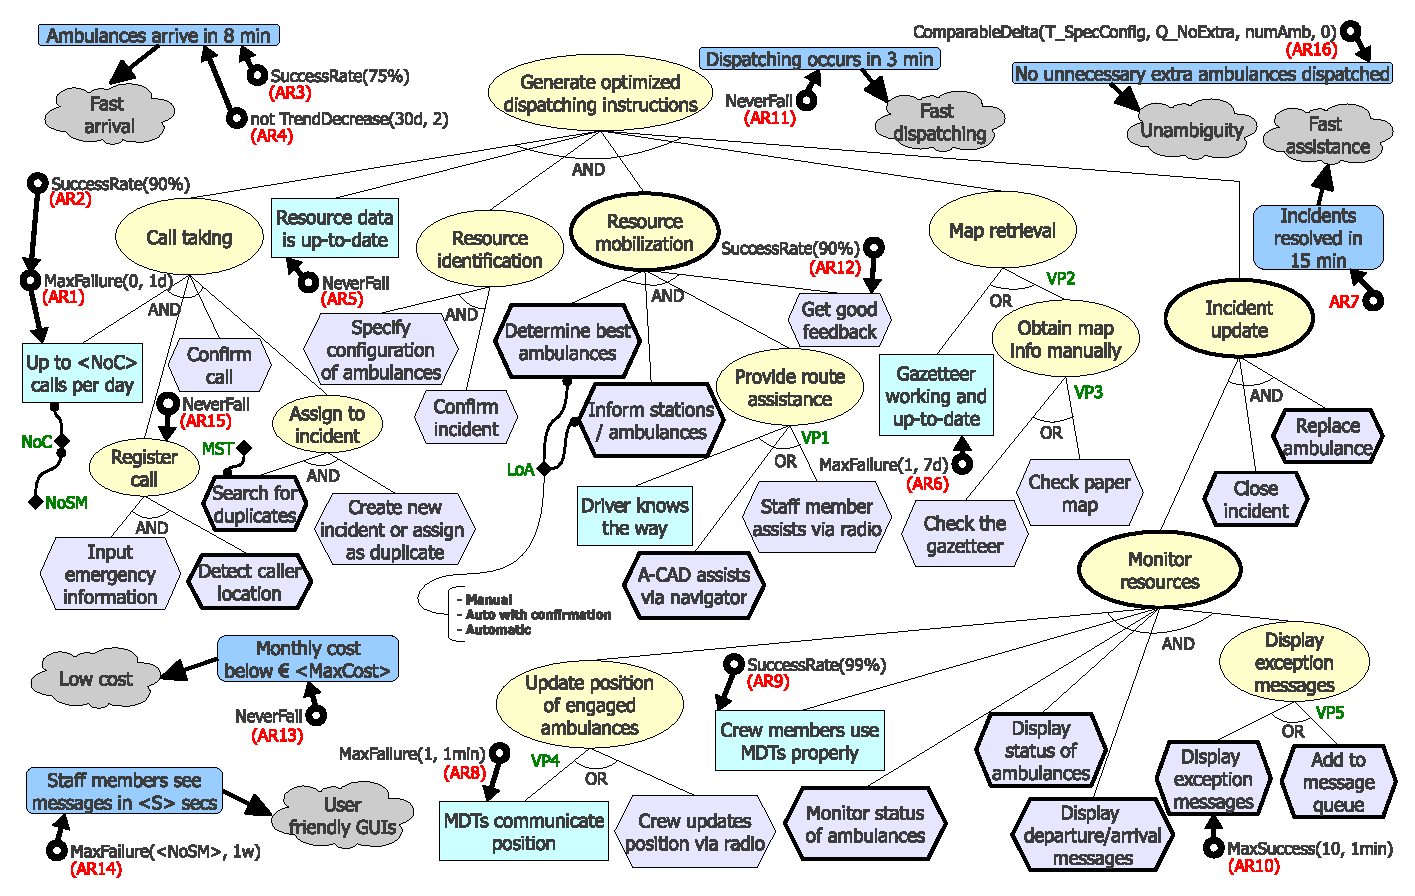
\includegraphics[width=\textwidth]{figuras/fig-intro-exemplosideways} 
	\caption{Exemplo de figura em modo paisagem: um modelo de objetivos~\cite{souza-mylopoulos:spe13}.}
	\label{fig-intro-exemplosideways}
\end{sidewaysfigure}



%%% Início de seção. %%%
\section{Tabelas}
\label{sec-intro-tabelas}

Tabelas são um ponto fraco do \latex. Elas são complicadas de fazer e, dependendo da complexidade da tabela (muitas células mescladas, por exemplo), vale a pena construi-las em outro programa (por exemplo, em seu editor de texto favorito) e inclui-las no documento como figuras. Mostramos, no entanto, alguns exemplos de tabela a seguir. O código utilizado para criar as tabelas encontra-se nas listagens~\ref{lst-intro-tabelas01}, \ref{lst-intro-tabelas02} e~\ref{lst-intro-tabelas03}.

\lstinputlisting[label=lst-intro-tabelas01, caption=Código \latex utilizado para inclusão das tabelas~\ref{tbl-intro-exemplo01} e~\ref{tbl-intro-exemplo02}., float=htpb]{codigos/lst-intro-tabelas01.tex}

\lstinputlisting[label=lst-intro-tabelas02, caption=Código \latex utilizado para inclusão da Tabela~\ref{tbl-intro-exemplo03}., float=htpb]{codigos/lst-intro-tabelas02.tex}

\lstinputlisting[label=lst-intro-tabelas03, caption=Código \latex utilizado para inclusão da Tabela~\ref{tbl-intro-exemplo04}., float=htpb]{codigos/lst-intro-tabelas03.tex}

Em particular, a Tabela~\ref{tbl-intro-exemplo04} utiliza um pacote chamado \texttt{tabularx}, que permite maior controle do layout das tabelas. Ao definir o ambiente \texttt{\textbackslash begin\{tabularx\}}, são definidos os tamanhos de cada coluna proporcional à largura ocupada pela tabela. Veja na Listagem~\ref{lst-intro-tabelas03} que as primeiras duas colunas não definem o atributo \texttt{\textbackslash hsize}, o que faz com que elas fiquem com o tamanho padrão de coluna, que é a largura da tabela dividida pelo número de colunas. Já a terceira coluna define \texttt{\textbackslash hsize=1.2\textbackslash hsize}, ou seja, esta coluna deve ser 20\% maior do que o tamanho padrão. Para isso, é preciso retirar de outras colunas, portanto a quarta e quinta colunas são definidas como 10\% menores (ou seja, \texttt{\textbackslash hsize=0.9\textbackslash hsize}).

% Exemplo de tabela 01:
\begin{table}
	\caption{Exemplo de tabela com diferentes alinhamentos de conteúdo.}
	\label{tbl-intro-exemplo01}
	\centering
	\begin{tabular}{ | c | l | r | p{40mm} |}\hline
		\textbf{Centralizado} & \textbf{Esquerda} & \textbf{Direita} & \textbf{Parágrafo}\\\hline
		C & L & R & Alinhamento de tipo parágrafo especifica largura da coluna e quebra o texto automaticamente.\\
		\hline
		Linha 2 & Linha 2 & Linha 2 & Linha 2\\
		\hline
	\end{tabular}
\end{table}

% Exemplo de tabela 02:
\begin{table}
	\caption{Exemplo que especifica largura de coluna e usa lista enumerada (adaptada de~\cite{souza-mylopoulos:spe13}).}
	\label{tbl-intro-exemplo02}
	\centering
	\renewcommand{\arraystretch}{1.2}
	\begin{small}
		\begin{tabular}{ | p{15mm} | p{77mm} | p{55mm} |}\hline
			\textbf{\textit{AwReq}} & \textbf{Adaptation strategies} & \textbf{Applicability conditions}\\\hline
			
			AR1 &
			\vspace{-2mm}\begin{enumerate}[topsep=0cm, partopsep=0cm, itemsep=0cm, parsep=0cm, leftmargin=0.5cm]
				\item \textit{Warning(``AS Management'')}
				\item \textit{Reconfigure($\varnothing$)}
			\end{enumerate}\vspace{-4mm} &
			\vspace{-2mm}\begin{enumerate}[topsep=0cm, partopsep=0cm, itemsep=0cm, parsep=0cm, leftmargin=0.5cm]
				\item Once per adaptation session;
				\item Always.
			\end{enumerate}\vspace{-4mm}
			\\\hline
			
			AR2 &
			\vspace{-2mm}\begin{enumerate}[topsep=0cm, partopsep=0cm, itemsep=0cm, parsep=0cm, leftmargin=0.5cm]
				\item \textit{Warning(``AS Management'')}
				\item \textit{Reconfigure($\varnothing$)}
			\end{enumerate}\vspace{-4mm} &
			\vspace{-2mm}\begin{enumerate}[topsep=0cm, partopsep=0cm, itemsep=0cm, parsep=0cm, leftmargin=0.5cm]
				\item Once per adaptation session;
				\item Always.
			\end{enumerate}\vspace{-4mm}
			\\\hline
		\end{tabular}
	\end{small}
\end{table}

% Exemplo de tabela 03:
\begin{table}
	\caption{Exemplo que mostra equações em duas colunas (adaptada de~\cite{souza-mylopoulos:spe13}).}
	\label{tbl-intro-exemplo03}
	\centering
	\vspace{1mm}
	\fbox{\begin{minipage}{.98\linewidth}
			\begin{minipage}{0.51\linewidth}
				\vspace{-4mm}
				\begin{eqnarray}
				\Delta \left( I_{AR1} / NoSM \right) \left[ 0, maxSM \right] > 0\\
				\Delta \left( I_{AR2} / NoSM \right) \left[ 0, maxSM \right] > 0\\
				\Delta \left( I_{AR3} / LoA \right) < 0\\
				\end{eqnarray}
				\vspace{-6mm}
			\end{minipage}
			\hspace{2mm}
			\vline 
			\begin{minipage}{0.41\linewidth}
				\vspace{-4mm}
				\begin{eqnarray}
				\Delta \left( I_{AR11} / VP2 \right) < 0\\
				\Delta \left( I_{AR12} / VP2 \right) > 0\\
				\Delta \left( I_{AR6} / VP3 \right) > 0\\
				\end{eqnarray}
				\vspace{-6mm}
			\end{minipage}
	\end{minipage}}
\end{table}

% Exemplo de tabela 04:
\begin{table}[h]
	\caption{Exemplo que utiliza o pacote \texttt{tabularx}, extraído de um artigo ainda não publicado.}
	\label{tbl-intro-exemplo04}
	\centering\tiny\def\tabularxcolumn#1{m{#1}}
	\begin{tabularx}{\columnwidth}{ >{\centering}X | >{\centering}X | >{\hsize=1.2\hsize\centering}X | >{\hsize=0.9\hsize\centering}X | >{\hsize=0.9\hsize\centering\arraybackslash}X }
		\hline
		\textbf{Applied Criteria} & \textbf{Analyzed Content} & \textbf{Initial\\Occurrences} & \textbf{Final Results} & \textbf{Reduction (\%)} \\
		\hline
		Duplicate Removal & Title, authors and year & 903 & 420 & 54,84\% \\ 
		\hline 
		IC and ECs & Title, abstract and keywords & 420 & 130 & 69,05\% \\ 
		\hline 
		IC and ECs & Full text & 130 & 117 & 10\% \\ 
		\hline 
		Final Results & -- & 903 & 117 & 87,04\% \\ 
		\hline 
	\end{tabularx}
\end{table}
\vspace*{2cm}
\endgroup
% ==============================================================================
% Projeto de Sistema - Nome do Aluno
% Capítulo 2 - Plataforma de Desenvolvimento
% ==============================================================================
\chapter{Plataforma de Desenvolvimento}
\label{sec-plataforma}

\vitor{As tabelas abaixo devem ser adaptadas às tecnologias e ferramentas utilizadas pelo aluno. Foram já indicadas algumas tecnologias bastante utilizadas em disciplinas e projetos em que estou envolvido.}


%=======================================================================================================
%			Tabela de Plataforma de Desenvolvimento e Tecnologias Utilizadas
%=======================================================================================================

Na Tabela~\ref{tabela-plataforma} são listadas as tecnologias utilizadas no desenvolvimento da ferramenta, bem como o propósito de sua utilização.

\begin{table}[h]
	\centering	
	\vspace{0.5cm}
	\footnotesize
	\caption{Plataforma de Desenvolvimento e Tecnologias Utilizadas}	
	\label{tabela-plataforma}
	\begin{tabular}{|p{1.6cm}|c|p{5cm}|p{6.5cm}|}  \hline 
 		Tecnologia & Versão & Descrição & Propósito \\\hline 
 		
		Java EE & 7 & Conjunto de especificação de APIs e tecnologias, que são implementadas por programas servidores de aplicação. & Redução da complexidade do desenvolvimento, implantação e gerenciamento de aplicações Web a partir de seus componentes de infra-estrutura prontos para o uso. \\ \hline

		Java & 8 & Linguagem de programação orientada a objetos e independente de plataforma. & Escrita do código-fonte das classes que compõem o sistema. \\\hline
		
		JSF & 2.2.12 & API para a construção de interfaces de usuários baseada em componentes para aplicações Web & Criação das páginas Web e sua comunicação com as classes Java.  \\\hline  
		
		EJB & 4.0.9 & API para construção de componentes transacionais gerenciados por \textit{container}. & Implementação das regras de negócio em componentes distribuídos, transacionais, seguros e portáveis. \\\hline
		
		JPA & 2.1 & API para persistência de dados por meio de mapeamento objeto/relacional. & Persistência dos objetos de domínio sem necessidade de escrita dos comandos SQL. \\\hline
		
		CDI & 1.1 & API para injeção de dependências. & Integração das diferentes camadas da arquitetura. \\\hline
		
		Facelets & 2.0 &  API para definição de decoradores (\textit{templates}) integrada ao JSF. & Reutilização da estrutura visual comum às paginas, facilitando a manutenção do padrão visual do sistema. \\\hline
		
		PrimeFaces & 6.2 &  Conjunto de componentes visuais JSF \textit{open source}. & Reutilização de componentes visuais Web de alto nível. \\\hline
		
		MySQL Server & 8.0 & Sistema Gerenciador de Banco de Dados Relacional gratuito. & Armazenamento dos dados manipulados pela ferramenta. \\\hline
		
		WildFly & 13 & Servidor de Aplicações para Java EE. & Fornecimento de implementação das APIs citadas acima e hospedagem da aplicação Web, dando acesso aos usuários via HTTP. \\\hline
		
		Apache Ant & 1.9.14 & Biblioteca Java e ferramenta de comandos que permitem compilar, montar, testar e executar aplicativos Java. & Execução de argumentos de linha de comando. \\\hline
	\end{tabular}
\end{table}






%=======================================================================================================
%			Tabela de Softwares de Apoio ao Desenvolvimento do Projeto
%=======================================================================================================

\newpage
Na Tabela~\ref{tabela-software} vemos os softwares que apoiaram o desenvolvimento de documentos e também do código fonte.

\begin{table}[h]
	\centering	
	\vspace{0.5cm}
	\caption{Softwares de Apoio ao Desenvolvimento do Projeto}	
	\label{tabela-software}
	\begin{tabular}{|p{3cm}|c|p{5cm}|p{6cm}|}  \hline 
	
 		Tecnologia & Versão & Descrição & Propósito \\\hline 
 		 
		FrameWeb Editor & 1.0 & Ferramenta CASE do método FrameWeb. & Criação dos modelos de Entidades, Aplicação, Persistência e Navegação. \\\hline

		TeX Live  & 2018 & Implementadão do \LaTeX & Documentação do projeto arquitetural do sistema. \\\hline       
		
		Texmaker & 5.0.2 & Editor de LaTeX. &  Escrita da documentação do sistema, sendo usado o \textit{template} \textit{abnTeX}.\footnote{\url{http://www.abntex.net.br}.} \\\hline    

		Eclipse Java EE IDE for Web Developers & 4.8 & Ambiente de desenvolvimento (IDE) com suporte ao desenvolvimento Java EE. & Implementação, implantação e testes da aplicação Web Java EE. \\\hline 
		
		Apache Maven & 3.5 & Ferramenta de gerência/construção de projetos de software. & Obtenção e integração das dependências do projeto. \\\hline
	\end{tabular}
\end{table}


\chapter{Atributos de Qualidade e Táticas}
\label{sec-atributos}

Na Tabela~\ref{tabela-atributos} são listados os atributos de qualidade considerados neste projeto, com uma indicação se os mesmos são condutores da arquitetura ou não e as táticas a serem utilizadas para tratá-los.

\begin{table}[h]
	\centering	
	\vspace{0.5cm}
	\caption{Atributos de Qualidade e Táticas Utilizadas}	
	\label{tabela-atributos}
	\begin{tabular}{|p{3.5cm}|p{2cm}|p{1.9cm}|p{7cm}|}  \hline 
	
 		\rowcolor[rgb]{0.8,0.8,0.8} Categoria & Requisitos Não Funcionais & Condutor da Arquitetura & Tática \\\hline
 		
 		Facilidade de Aprendizado, Operabilidade & RNF02, RNF03 & Sim & • Facilitar a compreensão do usuário para que os conceitos chaves sejam entendidos  de forma intuitiva, possibilitando que os comandos do sistema sejam operados com mais eficiência. Para isso, o sistema deve possuir diálogos simples para que nenhuma dúvida seja gerada no momento da inserção das informações. \\\hline  
 		
		Segurança de Acesso & RNF01 & Sim & • Garantir que os dados estão acessíveis apenas para aqueles que estão autorizados a acessá-los, evitando acesso não autorizado ou modificação dos dados.\\ &&&• Autorizar usuários, usando as classes de usuários definidas no projeto. \\\hline
		
		Manutenibilidade, Portabilidade & RNF04, RNF05, RNF06, RNF07 & Sim & • Organizar a arquitetura da ferramenta segundo uma combinação de camadas e partições.\\ &&&• A camada de lógica de negócio deve ser organizada segundo o padrão Camada de Serviço.\\ &&&• A camada de gerência de dados deve ser organizada segundo o padrão DAO.\\ &&&• Separar a interface com o usuário do restante da aplicação, segundo o padrão MVC. \\\hline  
		
		Reusabilidade & RNF07 & Não & • Reutilizar componentes e frameworks existentes.\\ &&&• Desenvolver novos componentes para reuso, quando não houver componentes disponíveis e houver potencial para reuso. \\\hline	
 		
	\end{tabular}
\end{table}


\chapter{Arquitetura de Software}
\label{sec-arquitetura}

A arquitetura de software do sistema~\imprimirtitulo \,\,segue a arquitetura padrão sugerida pelo FrameWeb~\cite{souza:masterthesis07,souza-et-al:iism09} baseada no padrão Camada de Serviço~\cite{fowler:book02}. A Figura~\ref{figura-arquitetura-padrao} ilustra a arquitetura estabelecida pelo método FrameWeb.

\begin{figure}[h]
	\centering
	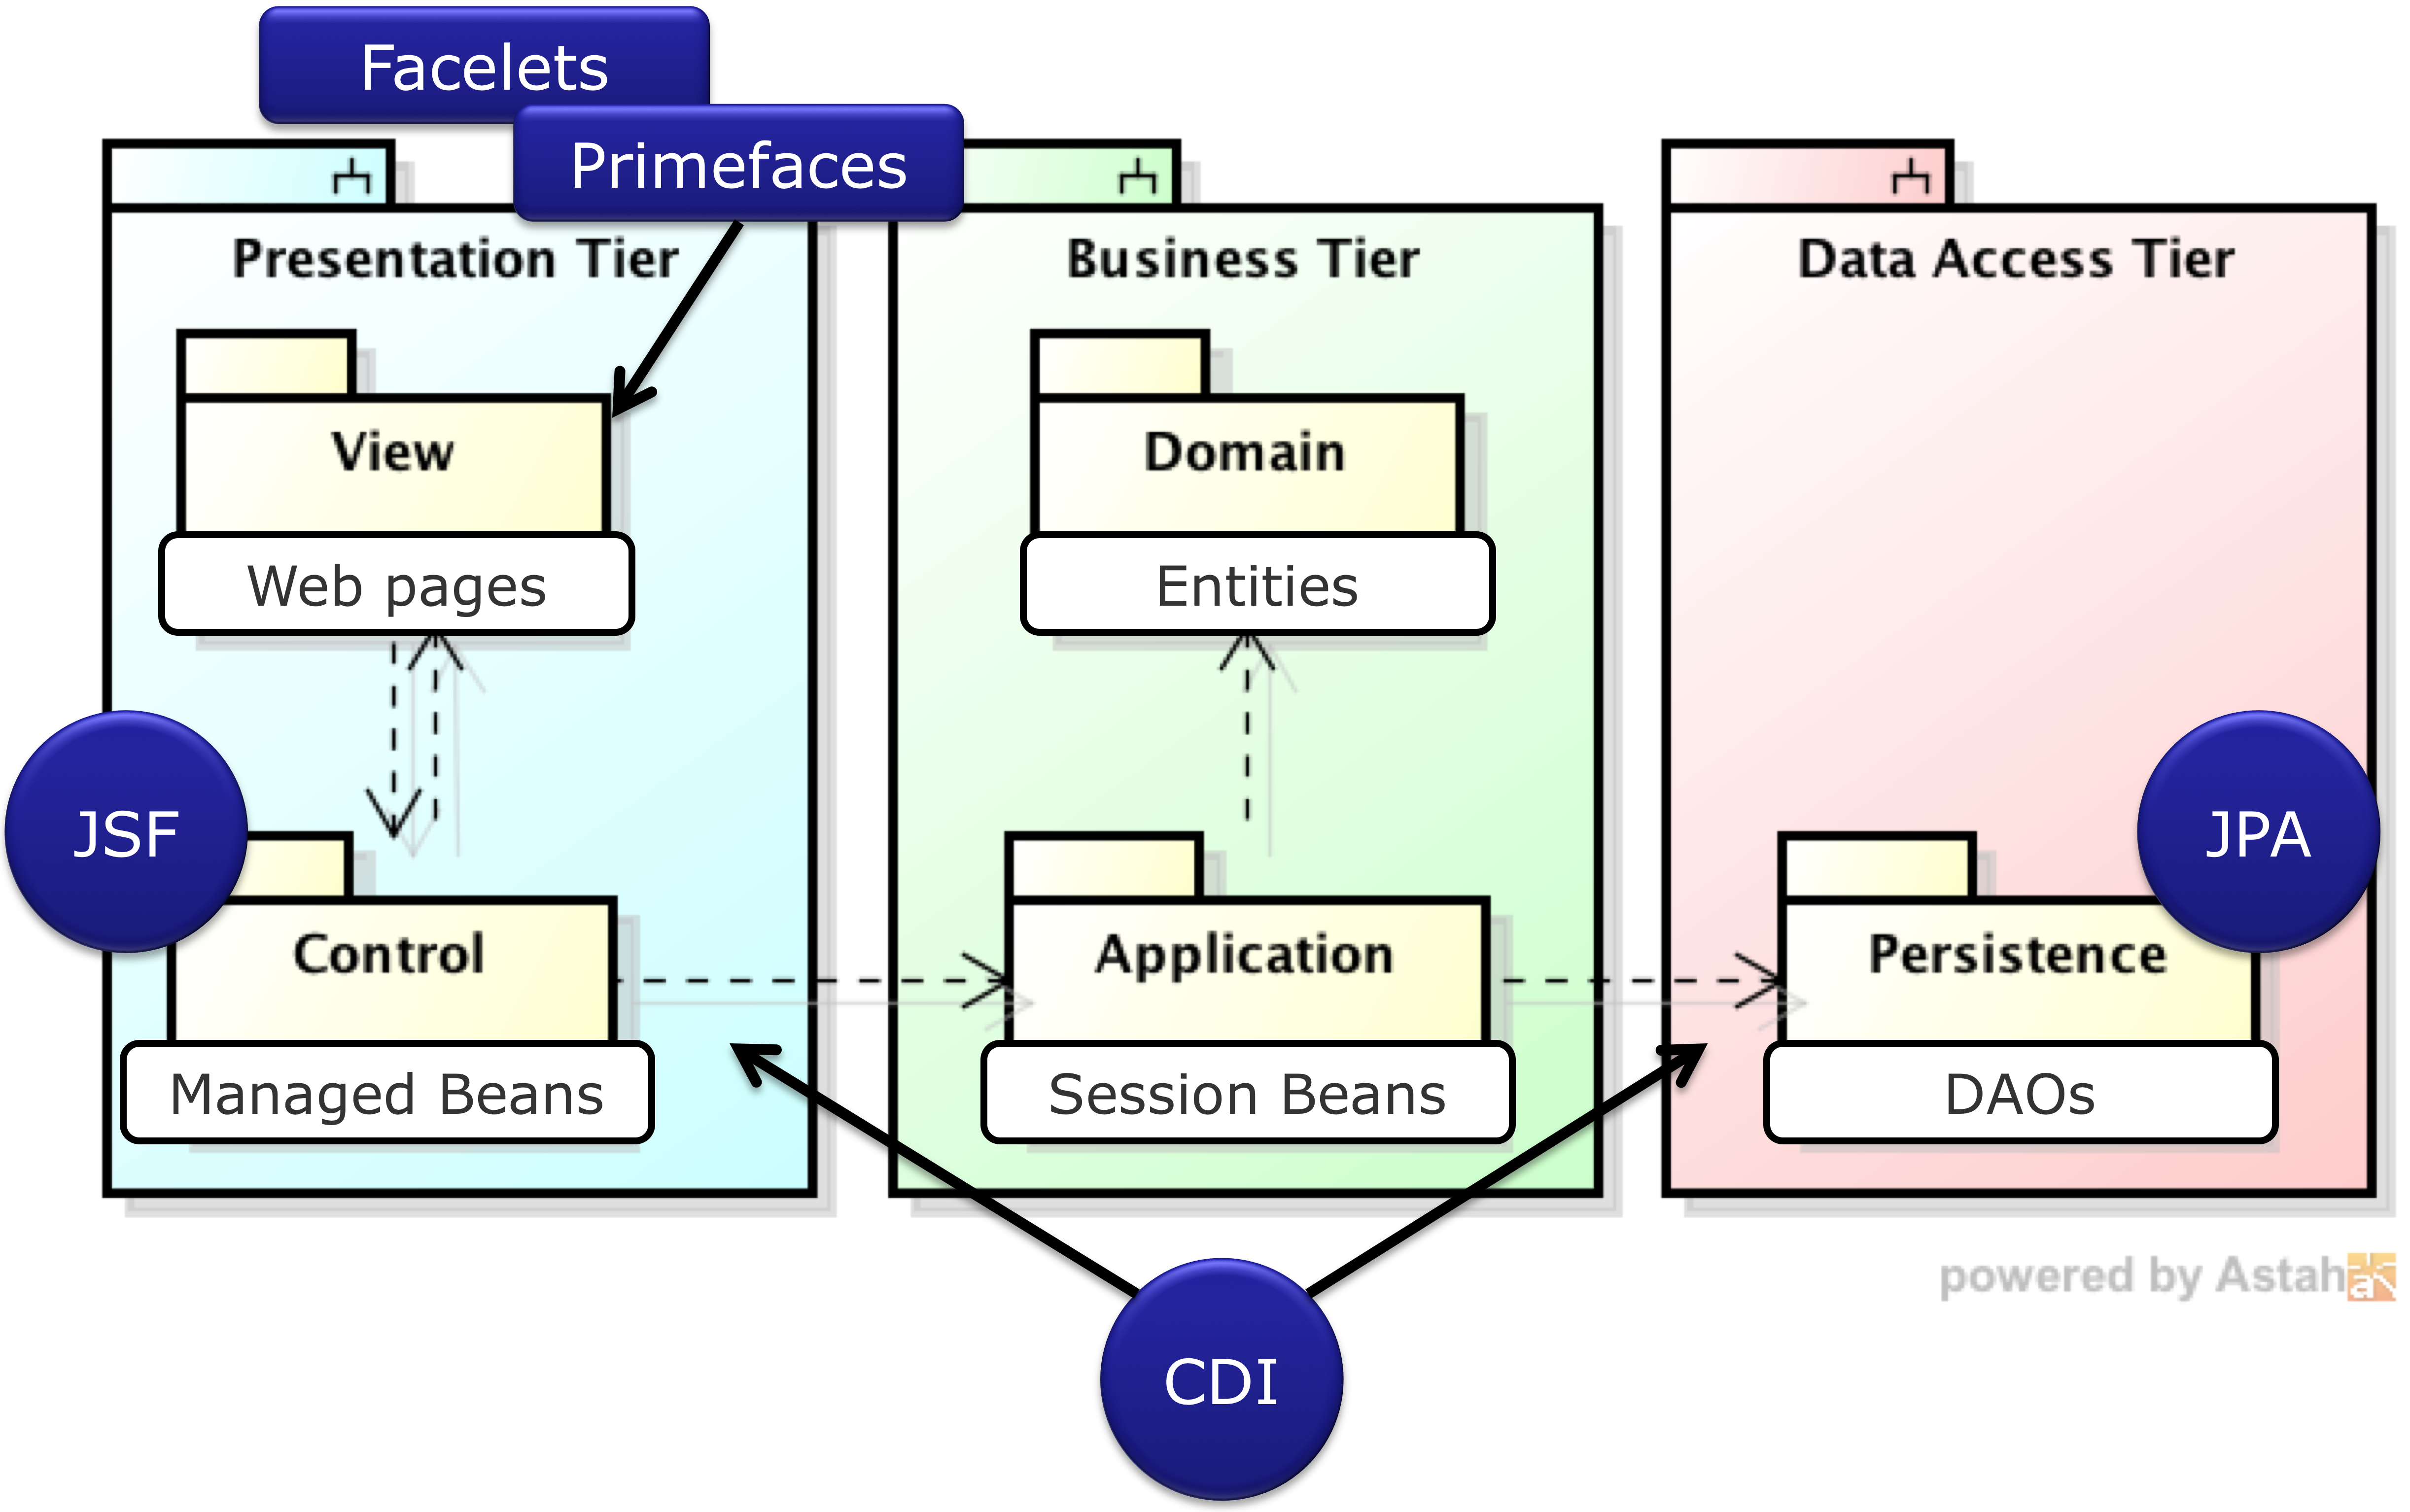
\includegraphics[width=0.8\textwidth]{figuras/figura-arquitetura-padrao.png}
	\caption{Arquitetura padrão proposta pelo FrameWeb.}
	\label{figura-arquitetura-padrao}
\end{figure}

Nas próximas seções, serão apresentados diagramas FrameWeb relativos a cada uma das camadas da arquitetura do sistema.


\section{Camada de Apresentação}
\label{sec-arquitetura-apresentacao}

\vitor{Apresentar os modelos de navegação do FrameWeb.}

\begin{figure}[h]
	\centering
	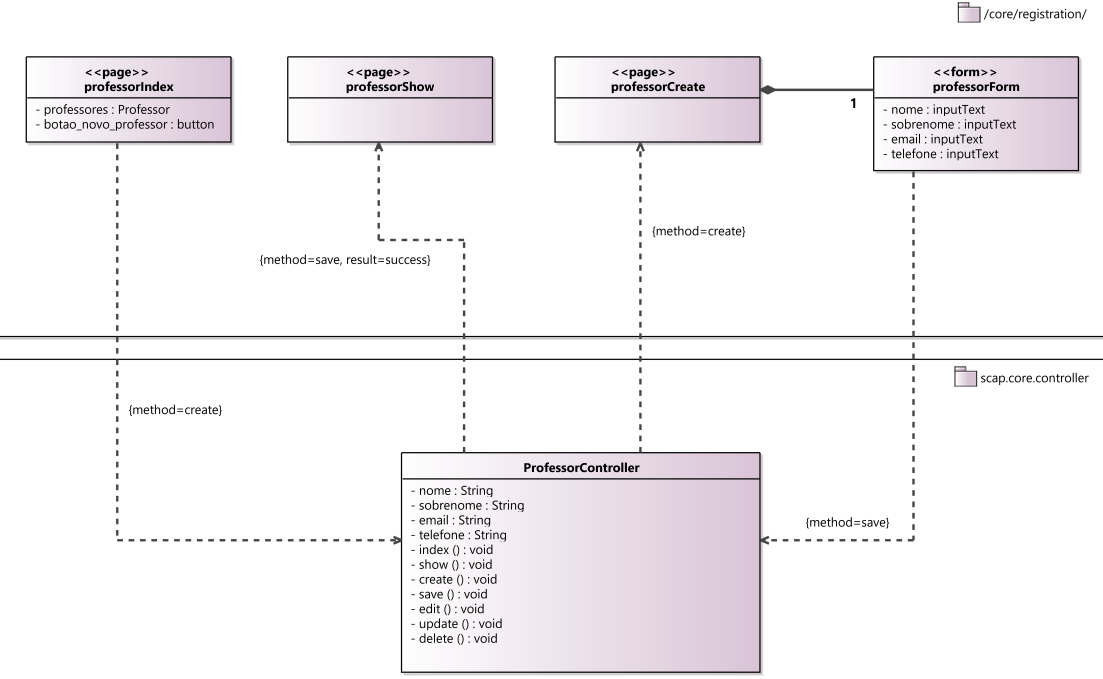
\includegraphics[width=1\textwidth]{figuras/figura-arquitetura-navegacao1.png}
	\caption{Modelo de Navegação do Caso de Uso: Cadastrar Usuário (Professor).}
	\label{figura-arquitetura-navegacao1}
\end{figure}

\begin{figure}[h]
	\centering
	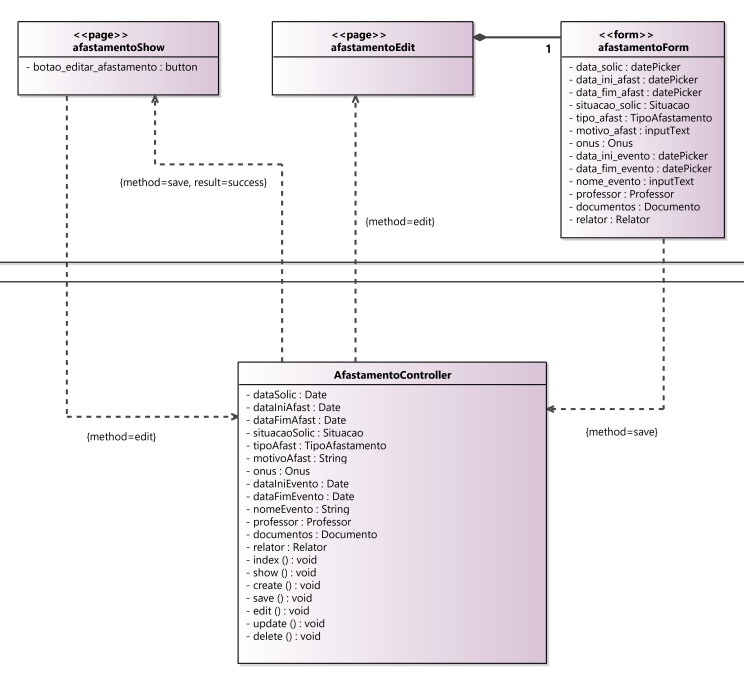
\includegraphics[width=1\textwidth]{figuras/figura-arquitetura-navegacao2.png}
	\caption{Modelo de Navegação do Caso de Uso: Arquivar Afastamento.}
	\label{figura-arquitetura-navegacao2}
\end{figure}

\section{Camada de Negócio}
\label{sec-arquitetura-negocio}

\vitor{Apresentar os modelos de entidades e de aplicação do FrameWeb.}

\begin{figure}[h]
	\centering
	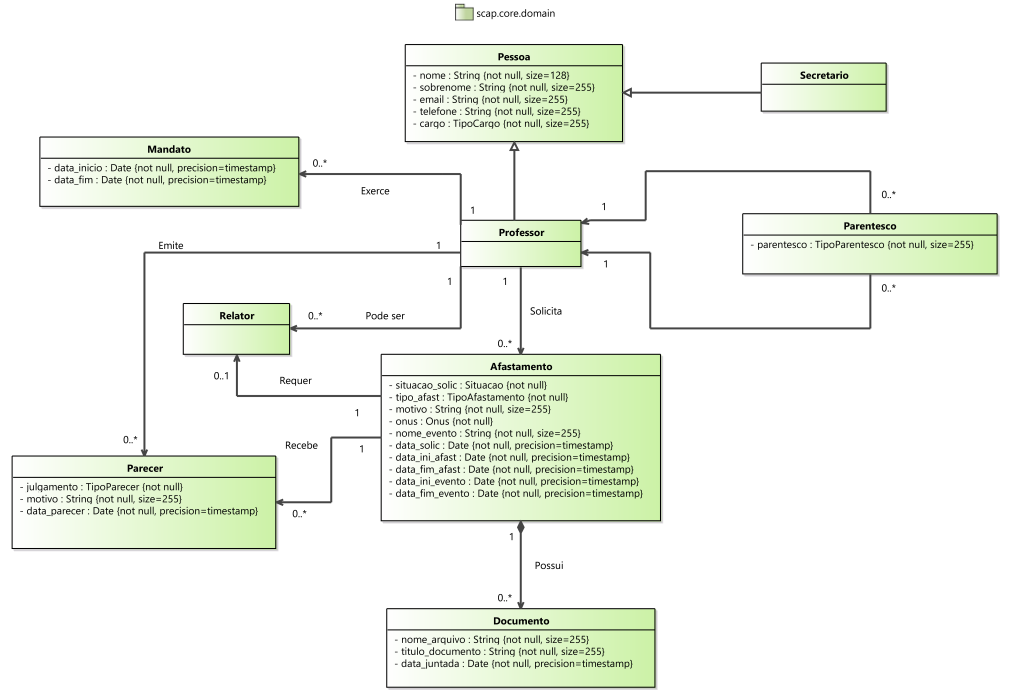
\includegraphics[width=1\textwidth]{figuras/figura-arquitetura-entidade.png}
	\caption{Modelo de Entidades.}
	\label{figura-arquitetura-entidade}
\end{figure}

\begin{figure}[h]
	\centering
	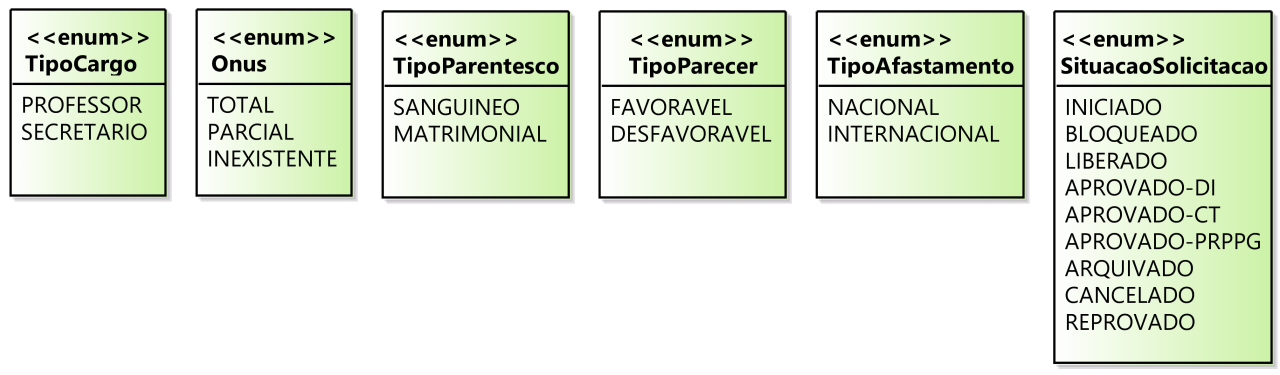
\includegraphics[width=1\textwidth]{figuras/figura-arquitetura-enum.png}
	\caption{Tipos Enumerados do SCAP.}
	\label{figura-arquitetura-enum}
\end{figure}

\begin{figure}[h]
	\centering
	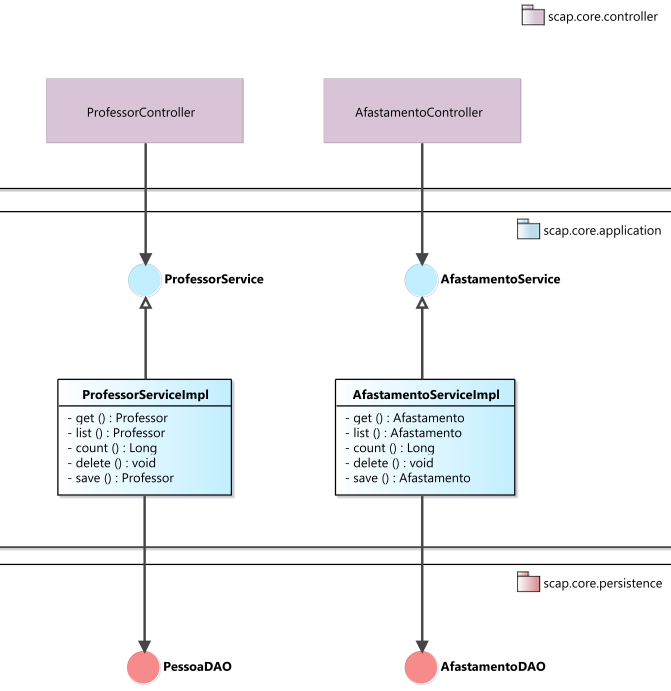
\includegraphics[width=1\textwidth]{figuras/figura-arquitetura-aplicacao.png}
	\caption{Modelo de Aplicação.}
	\label{figura-arquitetura-aplicacao}
\end{figure}

\section{Camada de Acesso a Dados}
\label{sec-arquitetura-dados}

\vitor{Apresentar os modelos de persistência do FrameWeb.}

\begin{figure}[h]
	\centering
	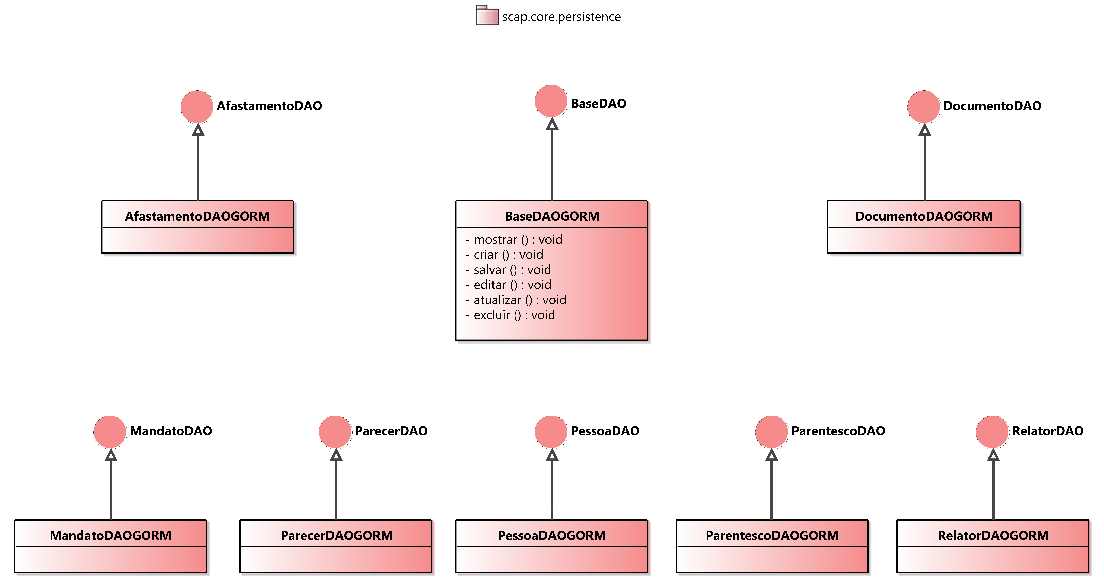
\includegraphics[width=1\textwidth]{figuras/figura-arquitetura-persistencia.png}
	\caption{Modelo de Persistência.}
	\label{figura-arquitetura-persistencia}
\end{figure}





%%% Páginas finais do documento: bibliografia e anexos. %%%
% Finaliza a parte no bookmark do PDF para que se inicie o bookmark na raiz e adiciona espaço de parte no sumário.
\phantompart

% Marca o início dos elementos pós-textuais.
\postextual

% Referências bibliográficas
\bibliography{bibliografia}

% Índice remissivo.
\phantompart
\printindex

% Fim do documento.
\end{document}
